\documentclass[12pt]{article}
\usepackage[T1]{fontenc}
\usepackage[utf8]{inputenc}
\usepackage{amsmath}
\usepackage[left=2cm,right=2cm,top=1cm,bottom=2cm]{geometry}
\usepackage{enumitem}
\usepackage{tikz}
\usepackage{multicol}
\usepackage{xcolor}

\pagestyle{empty}

% Boxen dicker gemacht
\newcommand{\answerbox}{\tikz \draw[line width=1.2pt] (0,0) rectangle ++(0.3cm,0.3cm);}
\newcommand{\filledbox}{\tikz \fill[black] (0,0) rectangle ++(0.3cm,0.3cm);}
\newcommand{\lightanswerbox}{\tikz \draw[line width=1.2pt, gray!30] (0,0) rectangle ++(0.3cm,0.3cm);}
\newcommand{\lightfilledbox}{\tikz \fill[gray!30] (0,0) rectangle ++(0.3cm,0.3cm);}

\begin{document}

{\color{gray!30}

\begin{center}
\textbf{\Huge Antwortblatt} \\
\vspace{0.3cm}
\textbf{Prüfung aus Quantitative Methoden 1, 17.12.25} \\
\vspace{0.3cm}
\textbf{\large MSc ZHAW}
\end{center}
\vspace{0.5cm}

\begin{tabular}{@{}p{0.5\textwidth}p{0.5\textwidth}@{}}
  Name: & Matrikelnummer: \\
  \vspace{5mm} & \vspace{5mm} \\
\end{tabular}

\vspace{10mm}

\noindent Identifikationsnummer:

\bigskip
}

% Boxen bleiben schwarz, nur Nummern darunter sind hellgrau
\noindent
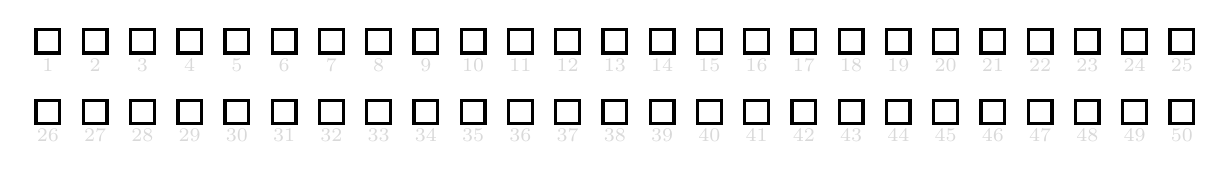
\begin{tikzpicture}[x=0.6cm, y=0.6cm]
  \foreach \x in {1,...,25} {
    \draw[line width=1.2pt] (\x, 0) rectangle +(0.5, 0.5);
    \node[gray!30] at (\x+0.25, -0.25) {\scriptsize \x};
  }
  \foreach \x in {26,...,50} {
    \draw[line width=1.2pt] ({(\x-25)}, -1.5) rectangle +(0.5, 0.5);
    \node[gray!30] at ({(\x-25)+0.25}, -1.75) {\scriptsize \x};
  }
\end{tikzpicture}

\vspace{5mm}

{\color{gray!30}
\noindent \textbf{Anweisungen:} Bitte färben Sie die richtigen Antworten in den dafür vorgesehenen Kästchen mit einem schwarzen Filzstift ein. \textbf{Nur} die hier angekreuzten Antworten werden gewertet (Fragen 1-25).\\
Anleitung, wie angekreuzt (ausgemalt) wird - \textbf{Korrekturen} werden auf diesem Blatt mit Tipp-Ex durchgeführt:

\begin{tabular}{cccc}
    \textcolor{gray!30}{A)} \lightfilledbox & \textcolor{gray!30}{B)} \lightanswerbox & \textcolor{gray!30}{C)} \lightfilledbox & \textcolor{gray!30}{D)} \lightanswerbox
\end{tabular}

\vspace{0.5cm}
}

\begin{multicols}{2}
\begin{enumerate}[itemsep=0.3cm, label={\textcolor{gray!30}{\arabic*.}}]
    % Linke Spalte: 12 Fragen
    \item \begin{tabular}{cccc} \textcolor{gray!30}{A)} \answerbox & \textcolor{gray!30}{B)} \answerbox & \textcolor{gray!30}{C)} \answerbox & \textcolor{gray!30}{D)} \answerbox \end{tabular}
    \item \begin{tabular}{cccc} \textcolor{gray!30}{A)} \answerbox & \textcolor{gray!30}{B)} \answerbox & \textcolor{gray!30}{C)} \answerbox & \textcolor{gray!30}{D)} \answerbox \end{tabular}
    \item \begin{tabular}{cccc} \textcolor{gray!30}{A)} \answerbox & \textcolor{gray!30}{B)} \answerbox & \textcolor{gray!30}{C)} \answerbox & \textcolor{gray!30}{D)} \answerbox \end{tabular}
    \item \begin{tabular}{cccc} \textcolor{gray!30}{A)} \answerbox & \textcolor{gray!30}{B)} \answerbox & \textcolor{gray!30}{C)} \answerbox & \textcolor{gray!30}{D)} \answerbox \end{tabular}
    \item \begin{tabular}{cccc} \textcolor{gray!30}{A)} \answerbox & \textcolor{gray!30}{B)} \answerbox & \textcolor{gray!30}{C)} \answerbox & \textcolor{gray!30}{D)} \answerbox \end{tabular}
    \item \begin{tabular}{cccc} \textcolor{gray!30}{A)} \answerbox & \textcolor{gray!30}{B)} \answerbox & \textcolor{gray!30}{C)} \answerbox & \textcolor{gray!30}{D)} \answerbox \end{tabular}
    \item \begin{tabular}{cccc} \textcolor{gray!30}{A)} \answerbox & \textcolor{gray!30}{B)} \answerbox & \textcolor{gray!30}{C)} \answerbox & \textcolor{gray!30}{D)} \answerbox \end{tabular}
    \item \begin{tabular}{cccc} \textcolor{gray!30}{A)} \answerbox & \textcolor{gray!30}{B)} \answerbox & \textcolor{gray!30}{C)} \answerbox & \textcolor{gray!30}{D)} \answerbox \end{tabular}
    \item \begin{tabular}{cccc} \textcolor{gray!30}{A)} \answerbox & \textcolor{gray!30}{B)} \answerbox & \textcolor{gray!30}{C)} \answerbox & \textcolor{gray!30}{D)} \answerbox \end{tabular}
    \item \begin{tabular}{cccc} \textcolor{gray!30}{A)} \answerbox & \textcolor{gray!30}{B)} \answerbox & \textcolor{gray!30}{C)} \answerbox & \textcolor{gray!30}{D)} \answerbox \end{tabular}
    \item \begin{tabular}{cccc} \textcolor{gray!30}{A)} \answerbox & \textcolor{gray!30}{B)} \answerbox & \textcolor{gray!30}{C)} \answerbox & \textcolor{gray!30}{D)} \answerbox \end{tabular}
    \item \begin{tabular}{cccc} \textcolor{gray!30}{A)} \answerbox & \textcolor{gray!30}{B)} \answerbox & \textcolor{gray!30}{C)} \answerbox & \textcolor{gray!30}{D)} \answerbox \end{tabular}
    
    \columnbreak
    
    % Rechte Spalte: 13 Fragen
    \item \begin{tabular}{cccc} \textcolor{gray!30}{A)} \answerbox & \textcolor{gray!30}{B)} \answerbox & \textcolor{gray!30}{C)} \answerbox & \textcolor{gray!30}{D)} \answerbox \end{tabular}
    \item \begin{tabular}{cccc} \textcolor{gray!30}{A)} \answerbox & \textcolor{gray!30}{B)} \answerbox & \textcolor{gray!30}{C)} \answerbox & \textcolor{gray!30}{D)} \answerbox \end{tabular}
    \item \begin{tabular}{cccc} \textcolor{gray!30}{A)} \answerbox & \textcolor{gray!30}{B)} \answerbox & \textcolor{gray!30}{C)} \answerbox & \textcolor{gray!30}{D)} \answerbox \end{tabular}
    \item \begin{tabular}{cccc} \textcolor{gray!30}{A)} \answerbox & \textcolor{gray!30}{B)} \answerbox & \textcolor{gray!30}{C)} \answerbox & \textcolor{gray!30}{D)} \answerbox \end{tabular}
    \item \begin{tabular}{cccc} \textcolor{gray!30}{A)} \answerbox & \textcolor{gray!30}{B)} \answerbox & \textcolor{gray!30}{C)} \answerbox & \textcolor{gray!30}{D)} \answerbox \end{tabular}
    \item \begin{tabular}{cccc} \textcolor{gray!30}{A)} \answerbox & \textcolor{gray!30}{B)} \answerbox & \textcolor{gray!30}{C)} \answerbox & \textcolor{gray!30}{D)} \answerbox \end{tabular}
    \item \begin{tabular}{cccc} \textcolor{gray!30}{A)} \answerbox & \textcolor{gray!30}{B)} \answerbox & \textcolor{gray!30}{C)} \answerbox & \textcolor{gray!30}{D)} \answerbox \end{tabular}
    \item \begin{tabular}{cccc} \textcolor{gray!30}{A)} \answerbox & \textcolor{gray!30}{B)} \answerbox & \textcolor{gray!30}{C)} \answerbox & \textcolor{gray!30}{D)} \answerbox \end{tabular}
    \item \begin{tabular}{cccc} \textcolor{gray!30}{A)} \answerbox & \textcolor{gray!30}{B)} \answerbox & \textcolor{gray!30}{C)} \answerbox & \textcolor{gray!30}{D)} \answerbox \end{tabular}
    \item \begin{tabular}{cccc} \textcolor{gray!30}{A)} \answerbox & \textcolor{gray!30}{B)} \answerbox & \textcolor{gray!30}{C)} \answerbox & \textcolor{gray!30}{D)} \answerbox \end{tabular}
    \item \begin{tabular}{cccc} \textcolor{gray!30}{A)} \answerbox & \textcolor{gray!30}{B)} \answerbox & \textcolor{gray!30}{C)} \answerbox & \textcolor{gray!30}{D)} \answerbox \end{tabular}
    \item \begin{tabular}{cccc} \textcolor{gray!30}{A)} \answerbox & \textcolor{gray!30}{B)} \answerbox & \textcolor{gray!30}{C)} \answerbox & \textcolor{gray!30}{D)} \answerbox \end{tabular}
    \item \begin{tabular}{cccc} \textcolor{gray!30}{A)} \answerbox & \textcolor{gray!30}{B)} \answerbox & \textcolor{gray!30}{C)} \answerbox & \textcolor{gray!30}{D)} \answerbox \end{tabular}
\end{enumerate}
\end{multicols}

\end{document}